\documentclass[a4paper,11pt]{article}
\title{GUIssing game}
\author{Izaak van Dongen}

% so the title can be accessed by fancyhdr (and is automatically correctly
% spelled etc)
\makeatletter
\let\thetitle\@title
\makeatother

% fonts
\usepackage[p,osf]{cochineal}
\usepackage[scale=.95,type1]{cabin}
\usepackage[cochineal,bigdelims,cmintegrals,vvarbb]{newtxmath}
% fixed width font with 80 chars per listing line
\usepackage[scaled=.94]{newtxtt}
\usepackage[cal=boondoxo]{mathalfa}

% make the document take up more of the page
\usepackage[margin=1in,headheight=13.6pt]{geometry}

% no paragraph indent
\usepackage[parfill]{parskip}

% custom document header/footer
\usepackage{fancyhdr}
\usepackage{lastpage}

\pagestyle{fancy}
\fancyhf{}
\lhead{\thetitle}
\rhead{Izaak van Dongen}
\rfoot{Page \thepage\ of \pageref{LastPage}}

% pretty table rules and multirow entries
\usepackage{booktabs}
\usepackage{multirow}

% plotting mathematical functions (needs version request)
\usepackage{pgfplots}
\pgfplotsset{compat=1.15}

% \url function and clickable table of contents. no ugly red boxes though
\usepackage[hidelinks]{hyperref}

% maths symbols and other stuff (supersedes the ams* packages)
\usepackage{mathtools}

% For framing definitions
\usepackage[framemethod=tikz]{mdframed}
\usepackage[most]{tcolorbox}

\newtcolorbox{definition}{
freelance,
before=\par\vspace{2\bigskipamount}\noindent,
after=\par\bigskip,
frame code={
  \node[
  anchor=south west,
  inner xsep=8pt,
  xshift=8pt,
  rounded corners=5pt,
  font=\bfseries\color{white},
  fill=gray] at (frame.north west) (tit) {\strut Definition:};
  \draw[
  line width=3pt,
  rounded corners=5pt,gray
  ] (tit.west) -| (frame.south west) -- ([xshift=15pt]frame.south west);
},
interior code={},
top=2pt
}

% for better table of contents stuff, providing the \listof* commands and not
% listing the tables in the table of contents
\usepackage[nottoc,notlof,notlot]{tocbibind}

% more advanced handling of utf8 and fonts or something. apparently good to have
\usepackage[utf8]{inputenc}
\usepackage[T1]{fontenc}

% bibliography management with square braces for citations
\usepackage[square]{natbib}

% graphics, like eps files and stuff (supersedes graphics)
\usepackage{graphicx}

% used to horizontally align floats
\usepackage{subfig}

% used for figures
\usepackage{float}

% needed for colouring and stuff (xcolor supersedes color)
\usepackage{xcolor}

\definecolor{codegreen}{rgb}{ 0,0.6,0}

% listings of code
\usepackage{minted}
\setminted{breaklines,
           breakbytokenanywhere,
           linenos
}
\usemintedstyle{friendly}
% bigger line numbers
\renewcommand\theFancyVerbLine{\footnotesize\arabic{FancyVerbLine}}

% that can break across pages while being captioned figures
\usepackage{caption}
\newenvironment{longlisting}
{\addvspace{\baselineskip}\captionsetup{type=listing}}
{\addvspace{\baselineskip}}

% allow maths to break across pages
\allowdisplaybreaks

\begin{document}
    \maketitle\thispagestyle{empty} % no page number under title
    \tableofcontents
    \listoflistings

    \section{Introduction}

    This project is the sequel to the popular \texttt{assignment\_guessing},
    at \url{https://github.com/elterminad0r/assignment_guessing}, now featuring
    a very useful and fluid graphical interface.

    It uses the same techniques to search both $\mathbb{Q}$ and $\mathbb{Z}$,
    but doesn't implement the linear approach to either, as it's not really
    preferable in any circumstance.

    \section{Programs}

    \subsection{Abstract}

    Despite the fact that the same algorithms from last time can be reapplied,
    their implementations have to be suited the the event-driven idiom. This is
    reflected in listing \ref{lst:guesser}, which contains the `boilerplate'
    code. It represents the broad protocol that a component implementing
    guessing should follow.

    This is that a guesser may must implement a method to ask a question, and a
    separate method that receives the answer. The guesser should appropriately
    modify its internal state so that it knows what question is being answered,
    and what to ask next. This is really a kind of poor man's synchronous
    coroutine, as implemented for example by Python's generators, where the
    internal state is simply a stack frame. However, these do not come with fpc.

    The other thing to note is that a guesser being able to deduce a number is
    considered exceptional behaviour, and hence is implemented by an exception,
    which should carry a message including what the correctly guessed number is,
    which may then be caught. If the guesser is not sure of the user's number,
    it should simply ask a normal question to verify if a guess is correct. This
    is implemented for example in listing \ref{lst:sternbrocot}.

    It is implemented as an abstract class rather than as an interface because
    the main code also wants to be able to tear the engine down, with a
    \texttt{Free} call to prevent memory leakage. Unfortunately, destructors
    can't be included in interfaces, so there is no guarantee that an
    implementing class can be freed. Because of this, I instead use an object,
    which \textit{is} understood to have a \texttt{Free} method.

\begin{longlisting}
\inputminted{Pascal}{../UGuesser.pas}
\caption{UGuesser.pas: Boilerplate and definitions for guessing objects}
\label{lst:guesser}
\end{longlisting}

    Listing \ref{lst:binary} shows a class implementing this protocol, namely by
    performing a binary search. As previously discussed, this version of binary
    search works on the entirety of $\mathbb{Z}$, by determining bounds in a
    similar `binary' manner (at least, it should be able to find sensible bounds
    in $O(\log_2(n))$ (and then guess the number in $O(\log_2(n))$).

\begin{longlisting}
\inputminted{Pascal}{../UBinarySearch.pas}
\caption{UBinarySearch.pas: Implementation of unbounded binary search}
\label{lst:binary}
\end{longlisting}

    Listing \ref{lst:sternbrocot} shows a class implementing a search on
    $\mathbb{Q}$. This is separated from listing \ref{lst:binary} as when
    considering the case of integers, this effectively degenerates into a slow
    linear search (taking the consecutive upper mediants of $\frac{0}{1}$ and
    $\frac{1}{0}$ results in the sequence $\frac{1}{1}$, $\frac{2}{1}$,
    $\frac{3}{1}$\ldots).

\begin{longlisting}
\inputminted{Pascal}{../USternBrocotSearch.pas}
\caption{USternBrocotSearch.pas: Implementation of unbounded rational search}
\label{lst:sternbrocot}
\end{longlisting}

    Listing \ref{lst:dummy} shows a dummy class that just displays a message
    whenever it is queried. This is useful for the main form code to show a
    persistent message to the user while no other searching engine is
    instantiated.

\begin{longlisting}
\inputminted{Pascal}{../UDummyGuesser.pas}
\caption{UDummyGuesser.pas: Dummy message-displaying object}
\label{lst:dummy}
\end{longlisting}


    \subsection{Boring}

    Listing \ref{lst:lfm} contains an abridged version of the lfm (Lazarus
    Forms) file, serving as a brief summary of all that I did in the object
    inspector.

\begin{longlisting}
\inputminted{pascal}{UGUIssing.lfm}
\caption{(Heavily redacted) UGUIssing.lfm: Layout and programmatic properties of
Form elements}
\label{lst:lfm}
\end{longlisting}

    Listing \ref{lst:forms} shows the `main' code that deals with the
    \texttt{TForm}. This part implements all the callbacks specified for each
    form component, and relays the user's actions to the \texttt{TGuesser}
    currently in action.

    My favourite part of this section is \texttt{KeyIntercept}, which enables
    the user not to have to press any buttons or really use the GUI at all,
    upgrading its usefulness to near CLI levels.

\begin{longlisting}
\inputminted{Pascal}{../UGUIssing.pas}
\caption{UGUIssing.pas: Implementing the Forms functionality}
\label{lst:forms}
\end{longlisting}

    \section{Result}

    A screenshot of the application is shown in fig \ref{pic:app}. The colouring
    is not specifically set for this game, but is just my personal GTK theme
    (Arc-Dark), which is detected by Lazarus.

\begin{figure}[H]
\begin{center}
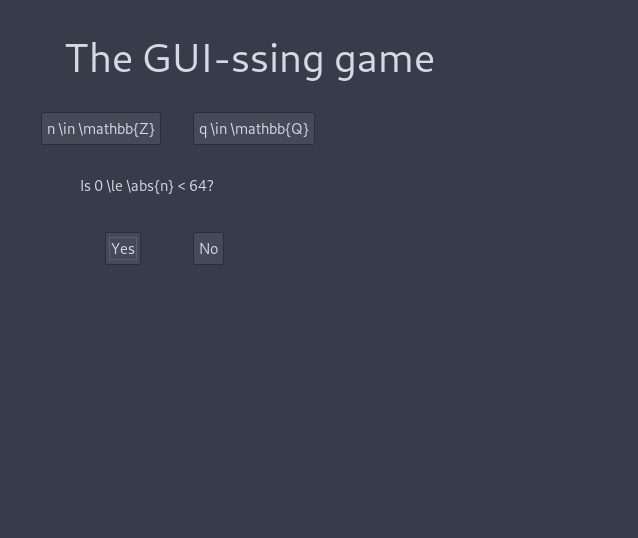
\includegraphics[width=0.5\textwidth]{win_screenshot_20180610_183143.png}
\end{center}
\caption{Screenshot of the game}\label{pic:app}
\end{figure}

    You may notice that all of the mathematics is formatted in the form of
    \LaTeX\ source. This is the second best way to format maths, beside rendered
    \LaTeX.

    The program can be interacted with by clicking the buttons, or, as covered
    earlier, by pressing the appropriate keys. Because of the various
    \mintinline{pascal}{writeln} statements I had included, I can easily capture
    the actions executed by the user and program without needing multiple
    screenshots. I first compiled using \texttt{lazbuild} or Lazarus, and then
    ran \mintinline{zsh}{./GUIssing > writeup/output.txt}. This produced the
    following file, after I executed a guess for
    $\forall S \in \{\mathbb{Z}, \mathbb{Q}\}$.

\begin{longlisting}
\inputminted{text}{output.txt}
\caption{Example session with program}
\end{longlisting}

    This demonstrates the program correctly feeding information between the user
    and the underlying search engine. I have performed several more tests,
    including the cases

    \begin{itemize}
    \item $0$
    \item $1$
    \item $-1$
    \item $200$
    \item $-130$
    \item $16$
    \end{itemize}
    in $\mathbb{Z}$, and
    \begin{itemize}
    \item $0$
    \item $1$
    \item $3$
    \item $-3$
    \item $\frac{4}{3}$
    \item $\frac{5}{2}$
    \item $-\frac{5}{2}$
    \end{itemize}
    in $\mathbb{Q}$. These were not included as entire logs as this would be a
    serious waste of paper.

    \section{Source}

    The full project in its directory structure, including this document (as a
    full-colour PDF and \TeX{} file), can be found at
    \url{https://github.com/elterminad0r/GUIssing}.

    I would also like to take this moment to apologise for the aesthetics of my
    previous PDFs, including the usage of the Computer Modern Font, but
    especially the fact that the code listings didn't use a proper fixed-width
    font.

\end{document}
